\let\negmedspace\undefined
\let\negthickspace\undefined
\documentclass[journal]{IEEEtran}
\usepackage[a5paper, margin=10mm, onecolumn]{geometry}
\usepackage{tfrupee}
\usepackage{gvv-book}
\usepackage{gvv}
\usepackage{cite}
\usepackage{amsmath,amssymb,amsfonts,amsthm}
\usepackage{algorithmic}
\usepackage{graphicx}
\usepackage{textcomp}
\usepackage{xcolor}
\usepackage{txfonts}
\usepackage{listings}
\usepackage{enumitem}
\usepackage{mathtools}
\usepackage{gensymb}
\usepackage{comment}
\usepackage[breaklinks=true]{hyperref}
\usepackage{tikz}
\usepackage{tkz-euclide} 
\usepackage{pgfplots}
\def\inputGnumericTable{}                                 
\usepackage[latin1]{inputenc}                                
\usepackage{color}                                            
\usepackage{array}                                            
\usepackage{longtable}                                       
\usepackage{calc}                                             
\usepackage{multirow}                                        
\usepackage{hhline}                                           
\usepackage{ifthen}                                           
\usepackage{lscape}

\begin{document}

\bibliographystyle{IEEEtran}
\vspace{3cm}

\title{10.3.5.4.2}
\author{EE24BTECH11011-B.PRANAY KUMAR}
{\let\newpage\relax\maketitle}

\renewcommand{\thefigure}{\theenumi}
\renewcommand{\thetable}{\theenumi}
\setlength{\intextsep}{10pt} 

\numberwithin{equation}{enumi}
\numberwithin{figure}{enumi}
\renewcommand{\thetable}{\theenumi}

\textbf{QUESTION} \\
A fraction becomes $\frac{1}{3}$ when 1 is subtracted from the numerator, and it becomes $\frac{1}{4}$ when 8 is added to its denominator. Find the fraction.\\

\textbf{SOLUTION} \\
Let the fraction be represented as $\frac{x}{y}$. From the given conditions:
\begin{align}
    \frac{x - 1}{y} &= \frac{1}{3} \\
    \frac{x}{y + 8} &= \frac{1}{4}
\end{align}

Rewriting the equations in matrix form $A\vec{x} = \vec{b}$:
\begin{align}
A &= \myvec{ 1 & -\frac{1}{3} \\ 1 & -\frac{1}{4} }\\
b &=  \myvec{ 1 \\ 0}
\end{align}

Performing LU decomposition:
\begin{align}
    A = L \cdot U,
\end{align}
where:
\begin{align}
    L &= \myvec{1 & 0 \\ \frac{3}{4} & 1}, \\
    U &= \myvec{1 & -\frac{1}{3} \\ 0 & -\frac{1}{12}}.
\end{align}

Factorization of LU:
Given a matrix $ \mathbf{A} $ of size $ n \times n $, LU decomposition is performed row by row and column by column. The update equations are as follows: \\
\quad 1. Start by initializing $ \mathbf{L} $ as the identity matrix $ \mathbf{L} = \mathbf{I} $ and $ \mathbf{U} $ as a copy of $ \mathbf{A} $.\\
\quad 2. For each column $ j \geq k $, the entries of $ U $ in the $ k $-th row are updated as:
\begin{align}
U_{k,j} = A_{k,j} - \sum_{m=1}^{k-1} L_{k,m} \cdot U_{m,j}\quad \forall \quad j \geq k
\end{align}
3. For each row $ i > k $, the entries of $ L $ in the $ k $-th column are updated as:
\begin{align}
L_{i,k} = \frac{1}{U_{k,k}} \brak{ A_{i,k} - \sum_{m=1}^{k-1} L_{i,m} \cdot U_{m,k}} \quad \forall \quad i > k
\end{align}

Solving $L\vec{y} = \vec{b}$ using forward substitution:
\begin{align}
    y_1 &= 1 \\
    \frac{3}{4} y_1 + y_2 &= 0\\
    y_2 &= -\frac{3}{4}
\end{align}

Thus:
\begin{align}
    \vec{y} = \myvec{1 \\ -\frac{3}{4}}.
\end{align}

Next, solving $U\vec{x} = \vec{y}$ using backward substitution:
\begin{align}
    -\frac{1}{12} y &= -\frac{3}{4} \\
    y &= 9\\
    x - \frac{y}{3} &= 1\\
    x &= 5
\end{align}

Hence, the fraction is $\frac{5}{12}$.

\begin{figure}[h!]
   \centering
   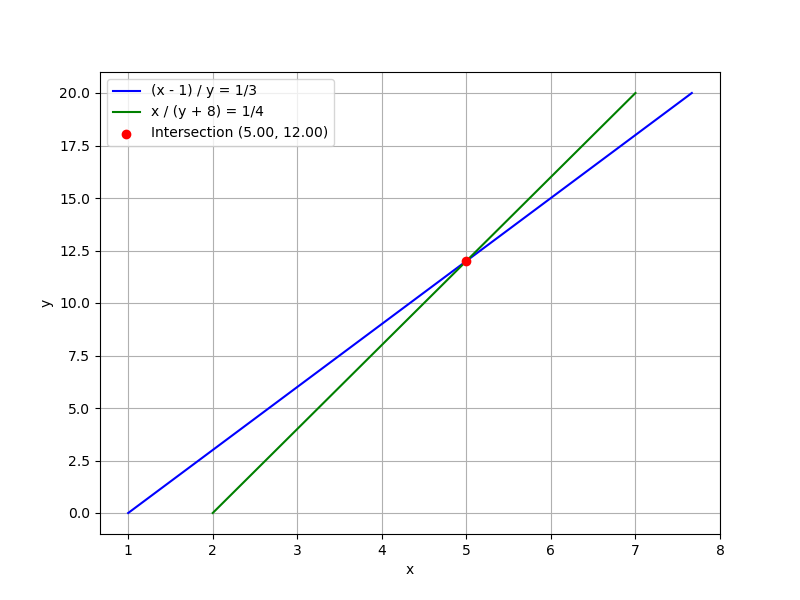
\includegraphics[width=1\columnwidth]{figs/fig.png}
    \caption{Solution to fraction problem using LU decomposition}
\end{figure}

\end{document}
